Mit wahnsinnigen Kopfschmerzen unerklärlichen Ursprungs haben wir \TOWN{Las Vegas} in Richtung Süden verlassen.
Auf dem Weg nach \TOWN{Palm Springs} liegt der National Park Joshua Tree, eine Wüste.
Gefrühstückt hatten wir in einem \FOREIGN{Diner} für deutlich weniger als am Vortag.
Gut gestärkt, eher überfressen, ging es zurück auf die Straße wobei ich zum ersten Mal das Steuer übernahm.
Das Fahren hier ist etwas anders als daheim.
Es gibt kein rechts vor links, sondern wer zuerst kommt mahlt zuerst.
Ebenso gibt es kein Rechtsfahrgebot, dadurch kann rechts wie links überholt werden und dann gibt es auf dem \FOREIGN{Highway} auch noch \FOREIGN{Crossing}s\footnote{Kreuzungen} (\FOREIGN{X-ING}) sowie Ampeln.
Die Geschwindigkeitsbeschränkung findet man sehr schnell angenehm, denn Überholmanöver sind dadurch sehr stressfrei und im Generellen muss man keine Bedenken haben, dass jemand von hinten angerauscht kommt.
Stellenweise lässt die Verfassung der Straße auch keine hohen Geschwindigkeiten zu.

Im Vergleich mit dem Grand Canyon ist der Joshua Tree National Park erstmal nicht so beeindruckend, aber auf eine andere Art doch ganz hübsch.
Vor allem ist es dort ruhig, weil weniger besucht.
Die angefahrene Aussichtsplattform (\FOREIGN{Keys West}) war zwar ein voller Reinfall, aber die auf dem Weg gelegenen Spots waren recht nett.
Denn diese bestanden i.d.R. aus Felsen, auf denen man herum klettern konnte und die waren wahnsinnig griffig!

Auf dem Weg nach \TOWN{Palm Springs} lagen dann noch ein paar Windräder\dots
Die Ortschaft liegt im \FOREIGN{Coachalla Valley} und dort findet jährlich das \glqq weltbekannte\grqq\, Coachalla Festival stattfindet.
In den 60er Jahren war \TOWN{Palm Springs} eine Erhohlungsstätte der amerikanischen Highsociety.
Heute ist der Ort im Endeffekt nur eine lang gezogene Hauptstraße mit Palmen.
Wirklich nicht der Rede wert.

\newpage
\thispagestyle{empty}
\begin{tikzpicture}[remember picture, overlay]
\node[inner sep=0pt, yshift=-.25\paperheight] at (current page.north) {%
	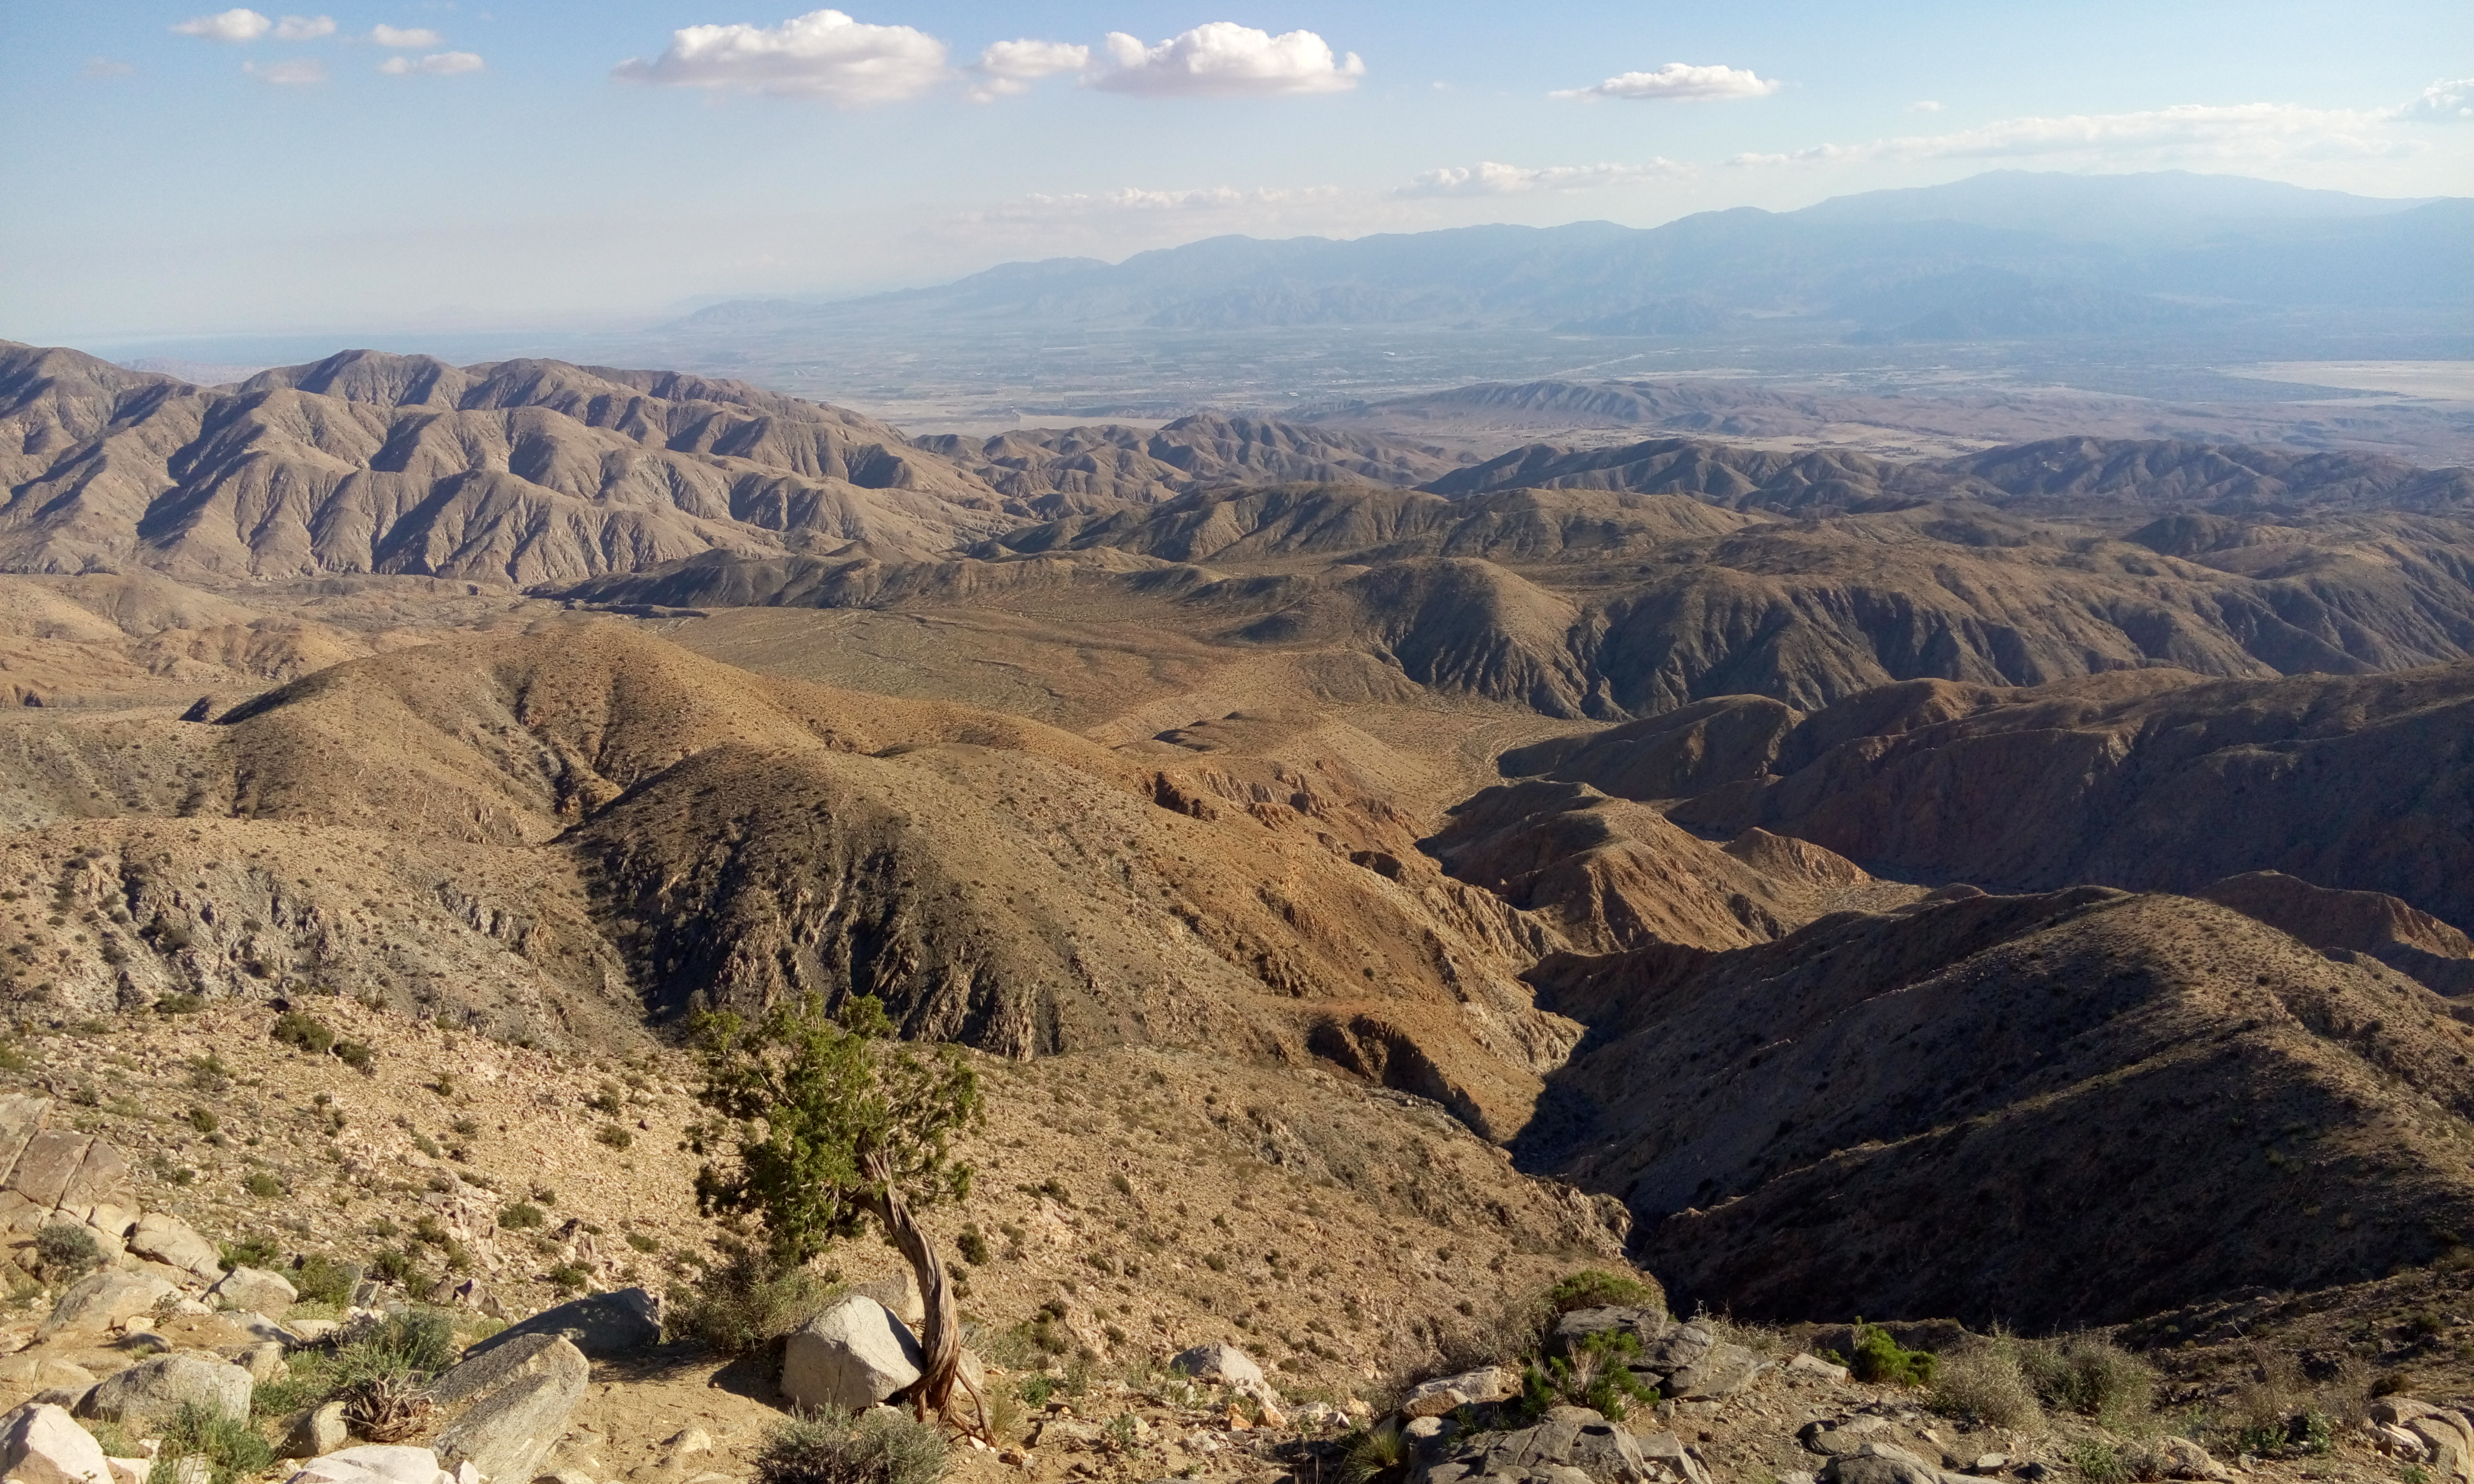
\includegraphics[width=\paperwidth,height=.5\paperheight]{12/image20160412_170805538.jpg};%
};
\node[inner sep=0pt, yshift=.25\paperheight] at (current page.south) {%
	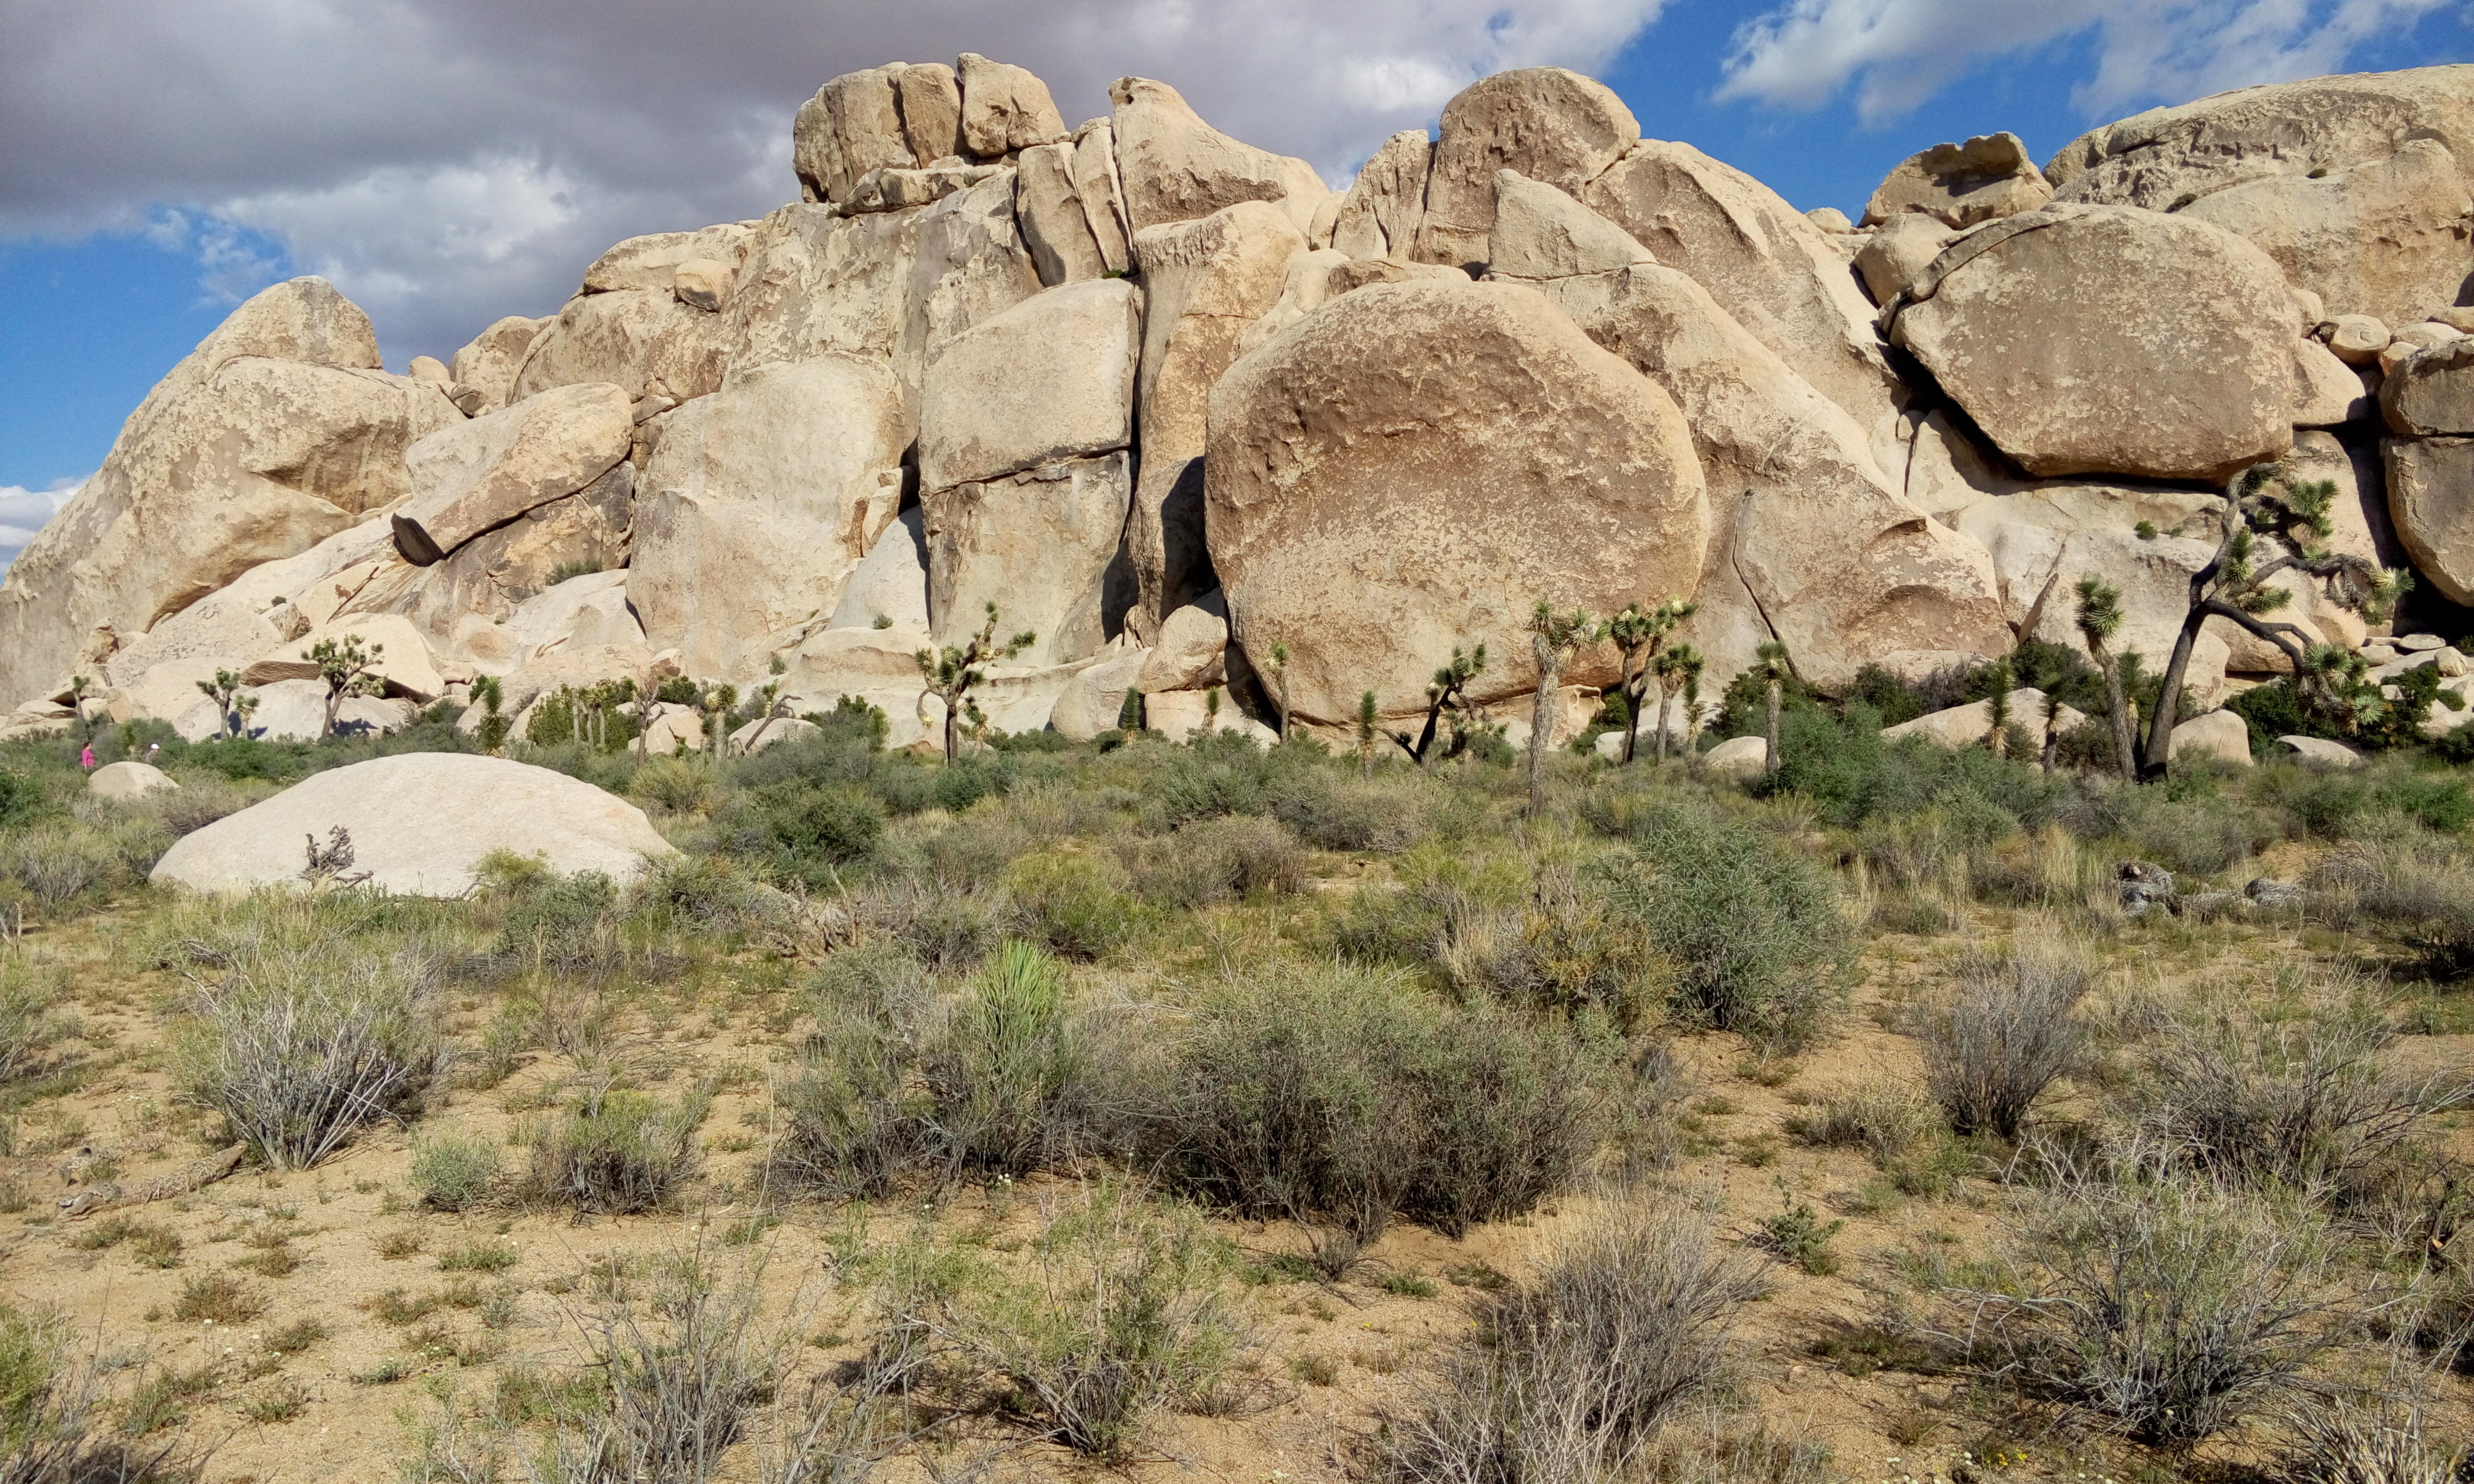
\includegraphics[width=\paperwidth,height=.5\paperheight]{12/image20160412_164403875.jpg};%
};
\end{tikzpicture}
\newpage
